\documentclass[a4paper,14pt]{extreport}
\usepackage[T2A]{fontenc}
\usepackage[utf8]{inputenc}
\usepackage{graphicx}
\usepackage{listings}
\usepackage[margin=0.7in]{geometry}
\usepackage{listings}
\usepackage{hyperref}
\usepackage{float}
\begin{document}
\begin{center}
\hfill \break
Университет ИТМО\\ 
Факультет ПИиКТ\\
\vspace{3in}
\huge{Лабораторная работа №2}\\
{по Компьютерной графике}\\
\vspace{2.5in}
\end{center}
\begin{flushright}
Выполнил:\\
Гуляев Б.С., Р3412
\end{flushright}
\vfill
\begin{center}
Санкт-Петербург, 2020
\end{center}
\thispagestyle{empty}
\newpage
\par \textbf{Цель}

Научиться работать с библиотекой OpenGL.

\par \textbf{Задание}

Средствами библиотеки OpenGL реализовать несколько типов источников света, движение камеры, динамику (движение некоторых объектов, например, снег). В центре сцены поставить объекты, на некоторые из них наложить текстуры. Объекты:
\begin{itemize}
    \item несколько различных примитивов, например, сферу, куб, тор.
    \item выгруженный из 3d редактора объект.
\end{itemize}

\par \textbf{Решение}

В ходе выполнения работы были реализованы 3 типа источников света:
\begin{enumerate}
    \item Ambient - с 10\%-яркостью освещены все поверхности
    \item Point - на сцене присутствует точечный источник света (маленький куб)
    \item Cone - тот же точечный источник света выступает в качестве источника напраленного луча света с ограниченным углом
\end{enumerate}

Движение камеры реализовано выбором направления через слежение за движением курсора, а также передвижением камеры с помощью клавиш со стрелкамив направлении относительном направления камеры.

В качестве динамичного объекта был создан куб, перемещающийся по окружности в плоскости X=0.

Всего на сцене присутствуют 4 фигуры:
\begin{enumerate}
    \item Кружащийся куб с текстурой 6-гранного кубика с разноцветными грянями
    \item Сфера с неподогнанной текстурой
    \item Модель низкополигональной лисы
    \item Маленький куб для обозначения источника света
\end{enumerate}

Кроме самой библиотеки OpenGL были использованы

\begin{itemize}
    \item библиотеки GLFW, GLEW и GLUT для работы с расширениями OpenGL
    \item библиотека stb\_image для загрузки изображений
    \item библиотека Assimp для импорта моделей
\end{itemize}

Расчет точек, нормалей и текстур для куба проводился вручную, для сферы - автоматизированно по формулам.
Модель лисы импортирована из формата OBJ.

Исходный текст программы можно получить по ссылке \url{https://github.com/bgs99/computer-graphics-lab2}

\begin{figure}[H]
    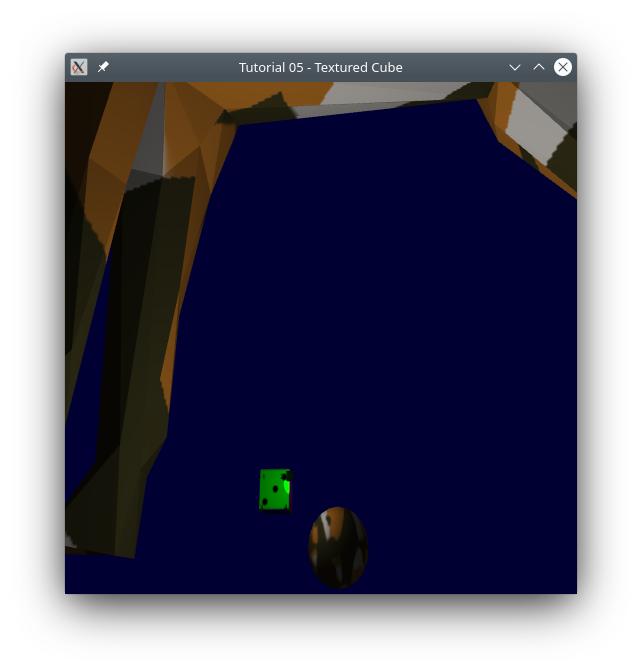
\includegraphics[width=\linewidth]{Screenshot.png}
    \caption{A screenshot of a working program}
    \label{fig:screen1}
\end{figure}

\par \textbf{Вывод}

В ходе выполнения данной лаораторной работы я создал простую интерактивную сцену с помощью библиотеки OpenGL, научился работать с шейдерами и разными видами освещения.

\end{document}
